\tikzstyle{block} = [draw, fill=blue!20, rectangle, 
    minimum height=3em, minimum width=6em]
\tikzstyle{block1} = [draw, fill=white!20, rectangle, 
    minimum height=3em, minimum width=10em]
\tikzstyle{pinstyle} = [pin edge={to-,think,black}]
\tikzstyle{input} = [coordinate]
\tikzstyle{output} = [coordinate]
\tikzstyle{line} = [ draw, dashed, line width = 0.5pt, -latex']
\begin{center}
\begin{minipage}{0.75\textwidth}
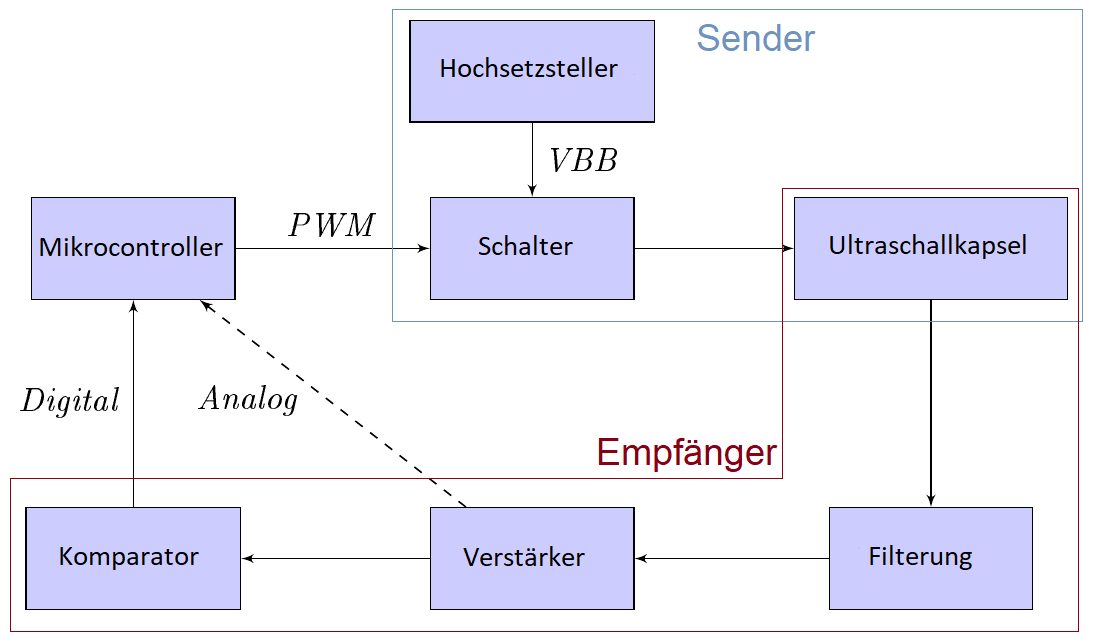
\includegraphics[width=1\textwidth%, draft
]{Abbildungen/Schema.png}
\captionof{figure}{Blockschaltbild des Ultraschall-Entfernungsmessers}
\label{fig:Blockschaltbild}
%\begin{tikzpicture}[auto, node distance=2cm,>=latex']
%\begin{picture}(250,100)
%%\put(-38,-122){\dashbox{2.5}(210,45)[rb] {Empfänger}}
%%\put(-38-122){\text{Empfänger}}
%\node [block](controller){Controller};
%\node [block, right of=controller, node distance=4.5cm] (schalter)  {Schalter};
%\node [block, above of=schalter, node distance=2cm] (hochsetzsteller) {Hochsetzsteller};
%\node [block, right of=schalter, node distance=4.5cm] (ultraschallkapsel)  {Ultraschallkapsel};
%\node [block, below of=ultraschallkapsel, node distance=3.5cm] (filterung)  {Filterung};
%\node [block, left of=filterung, node distance=4.5cm] (verstaerker)  {Verstaerker};
%\node [block, left of=verstaerker, node distance=4.5cm] (komperrator)  {Komperrator};
%
%\draw [->] (controller) -- node[name=PWM ] {$PWM$}  (schalter);
%\node [output, right of=schalter] (output) {};
%\coordinate [below of=PWM] (tmp);
%\draw [->] (hochsetzsteller) -- node[name=VBB ] {$VBB$}  (schalter);
%\node [output, above of=schalter] (output) {};
%\coordinate [below of=VBB] (tmp);
%\draw [->] (schalter) --  (ultraschallkapsel);
%\draw [->] (ultraschallkapsel) --  (filterung);
%\draw [->] (filterung) --  (verstaerker);
%\draw [->] (verstaerker) --  (komperrator);
%\node [output, right of=schalter] (output) {};
%\coordinate [below of=PWM] (tmp);
%\draw [->] (komperrator) --  node[name=Digital ] {$Digital$} (controller);
%\node [output, above of=komperrator] (output) {};
%\coordinate [below of=Digital] (tmp);
%\path[line] (verstaerker)--node[name=analog] {$Analog$}  (controller);
%\end{picture}
%\end{tikzpicture}
%\captionof{figure}{Blockschaltbild}
%\label{fig:Blockschaltbild1}

\end{minipage}
\end{center}
Die Abbildung \ref{fig:Blockschaltbild} zeigt eine vereinfachte Funktionsübersicht der Platine. Die Schaltpläne zu den verschiedenen Ausführungen der Platine sind den Anlagen beigefügt.

\subsection{Mikrocontroller}
Der Mikrocontroller soll eine stabile und variable PWM ausgeben können. Es werden für die Zeiterfassung und die PWM Ausgabe mehrere Timer benötigt, die sowohl intern als auch über die Hardware angesteuert werden können. Ein Analog/Digital-Wandler sollte ebenfalls vorhanden sein.

\subsection{Sender}
Der Sender soll Schallwellen im Ultraschallbereich (40\,kHz) aussenden. Diese sollen einen ausreichenden Schalldruck haben um von Hindernissen, die mehrere Meter entfernt sind, ein Echo erhalten zu können. Dafür muss die Ultraschallkapsel mit einem sinusähnlichen Signal angesteuert werden. Dessen Amplitude muss angemessen hoch sein, um den gewünschten Schalldruck zu erzeugen. Der Mikrocontroller ist auf eine Spannungsebene von 3,3\,V begrenzt. Um höhere Spannungen an der Ultraschallkapsel realisieren zu können, muss ein Schalter als weiteres Bauteil dazwischen geschaltet werden. Dieses zusätzliche Bauteil dient als Trennung zwischen den 3,3\,V des Mikrocontrollers und der höheren Spannungsebene der Lautsprecherkapsel. Dabei muss darauf geachtet werden, dass der Schalter schnell genug arbeitet, um die 40\,kHz auch zuverlässig schalten zu können.

\subsection{Hochsetzsteller}
Der Hochsetzsteller generiert aus den 5\,V Versorgungsspannung eine höhere Spannung für den Sendebetrieb. So kann der Schalldruck, der ausgegeben wird erhöht werden (größere Reichweite/größeres Rücksignal) siehe Abbildung \ref{fig:5v5m2}.\\
Die Funktionsweise des Hochsetzstellers (Spannungspumpe/Aufwärtswandler/Aufwärtsregler) ist überschaubar und findet in vielen Bereichen Anwendung. Grundsätzlich wird eine Induktivität in Reihe mit einer Freilaufdiode vor einen Ladekondensator geschaltet. Dieser liegt parallel zum Ausgang. Zwischen der Spule und der Diode ist ein Schalter angeschlossen, der die Spule gegen Masse schaltet. Die Spule lädt sich bei Betätigung des Schalters auf. Durch den Stromfluss entsteht ein Magnetfeld und beim öffnen steigt die Spannung am sekundären Ende der Spule. Durch das zusammenbrechende Magnetfeld an und lädt den Kondensator auf. Dieser Vorgang wird wiederholt bis der Kondensator so weit aufgeladen ist, dass die Ausgangsspannung den gewünschten Wert hält. Die mögliche Ausgangsspannung ist nicht unbegrenzt über das Schaltspiel regelbar. Sie ist von den Eigenschaften der Komponenten abhängig. 

\subsection{Ultraschallkapsel}
Für das Senden und Empfangen des Ultraschalls wird eine auf Piezomodulen basierende Ultraschallkapsel verwendet, weil Sie die Möglichkeit hat ein Signal auszugeben sowie zu empfangen und in Kleinbauform erhältlich ist. Wie stark das Nachschwingen der Kapsel eine Auswirkung auf die Empfängerschaltung hat, sowie die Größe der Störfrequenz bei verschiedenen Amplituden auf unterschiedlichen Entfernungen sollte überprüft werden. Es sollte auch getestet werden welche Kapseln sich für einen stand-alone Betrieb am besten eignen.

\subsection{Filter}
Die Filterschaltung soll am Eingang des Empfängers etwaig Störfrequenzen herauszufiltern um eine Verfälschung der gemessenen Strecke zu vermeiden, da die Ultraschallkapsel nicht ausschließlich Ultraschallsignale aufnimmt. Für hohe Frequenzen eignet sich eine passive Hochpassfilter-Schaltung, es wird zu einem Kondensator oder einer Spule ein Widerstand parallel zur Masse bestückt. 

\subsection{Empfänger}
Im Empfangsbetrieb werden die zurückkommenden Schallsignale, die auf die Ultraschallkapsel treffen, in sinusförmige Spannungssignale umgewandelt. Die Amplitude hängt von dem Schalldruck der empfangenen Signale ab und ist deutlich niedriger als die Amplitude der gesendeten Signale. Diese Signale müssen anschließend verstärkt werden, um sie mit dem Mikrocontroller auswerten zu können. Zur Vereinfachung der Auswertung wird das eingehende analoge Signal in ein digitales Signal umgewandelt, um Verarbeitungsaufwand einsparen zu können. Die Analyse eines Analogsignals erfordert mehr Programmieraufwand als die Auswertung eines Digitalsignals. Um die Qualität der gemessenen Entfernung besser zu beurteilen, sollte potenziell auch das Analogsignal ausgewertet und mit dem digitalen Signal verglichen werden. 












